\section{Aufgabe 6}
In dieser Aufgabe wird der Zufallsgenerator
\begin{equation}
  x_n = (a \cdot x_{n-1} + b) \% m  \rightarrow v_n = \frac{x_n}{m}\label{eqn:randon}
\end{equation}
untersucht. \\
Für die Teilaufgaben \ref{sec:6b} und \ref{sec:6c} werden die Werte $a=1601$, $b=3456$ und $m=10^4$ verwendet.
\subsection{Teilaufgabe a)}
Für den Zufallszahlengenerator \eqref{eqn:random} ergeben sich für für ein varaibles, ganzzahliges $a$, $b=3$, $m=1024$
und dem Startwert $x_0=0$ die in \ref{fig:periodenlänge} zu sehenden Periodenlängen.

\begin{figure}[H]
  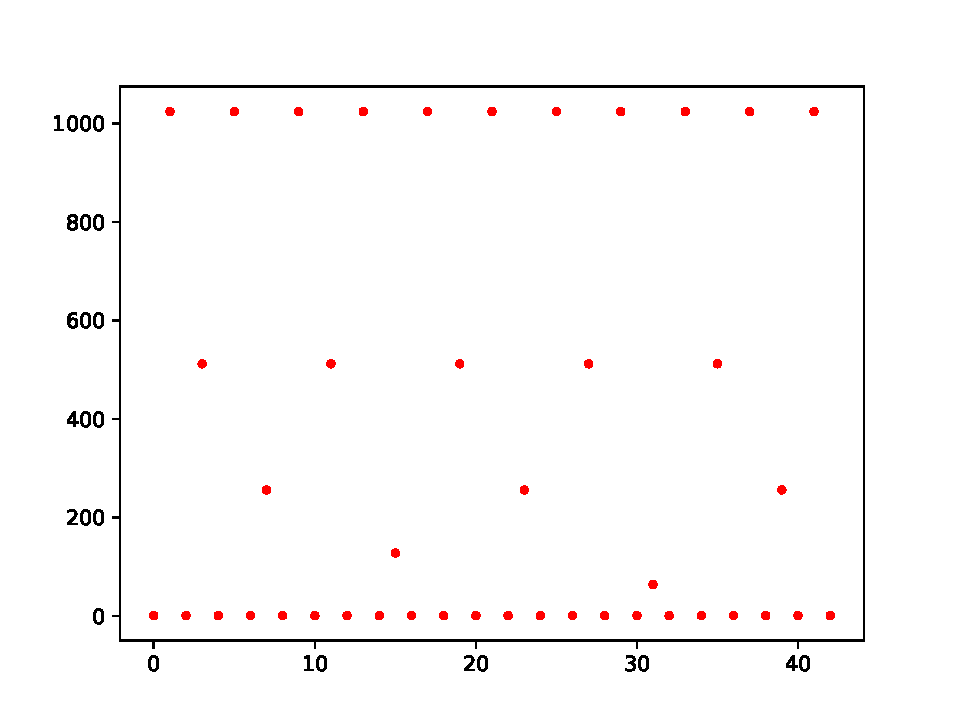
\includegraphics{Aufgabe06/Teilaufgabe_a).pdf}
  \caption{Periodenlängen in Abhängigkeit von a}
  \label{fig:periodenlänge}
\end{figure}

Es ist zu erkennen, dass bei $a=4 \cdot n + 1 $ die maximale Periodenlänge auftritt.
Das Ergebnis lässt sich mit den Regeln für gute linear-kongruente Generatoren erklären:
\begin{itemize}
  \item $b = 3 \neq 0$
  \item $b$ und $m$ sind Teilerfremd, da die Quersumme von $1024$ gleich $7$ ist. Daher ist $m$ nicht durch $b$ teilbar.
  \item Jeder Primfaktor von $m$ teilt $a-1$, da $1024=2^10$ und $a-1=4n$ mit $n \in \mathbb{N}$.
  \item $1024=2^10=4^5$, $a-1=4n$ $n \in \mathbb{N}$ \textrightarrow beide sind durch $4$ teilbar.
\end{itemize}

\subsection{Teilaufgabe b)} \label{sec:6b}
Für die gegebenen Startwerte ergibt sich folgendes Diagramm:
\begin{figure}[H]
  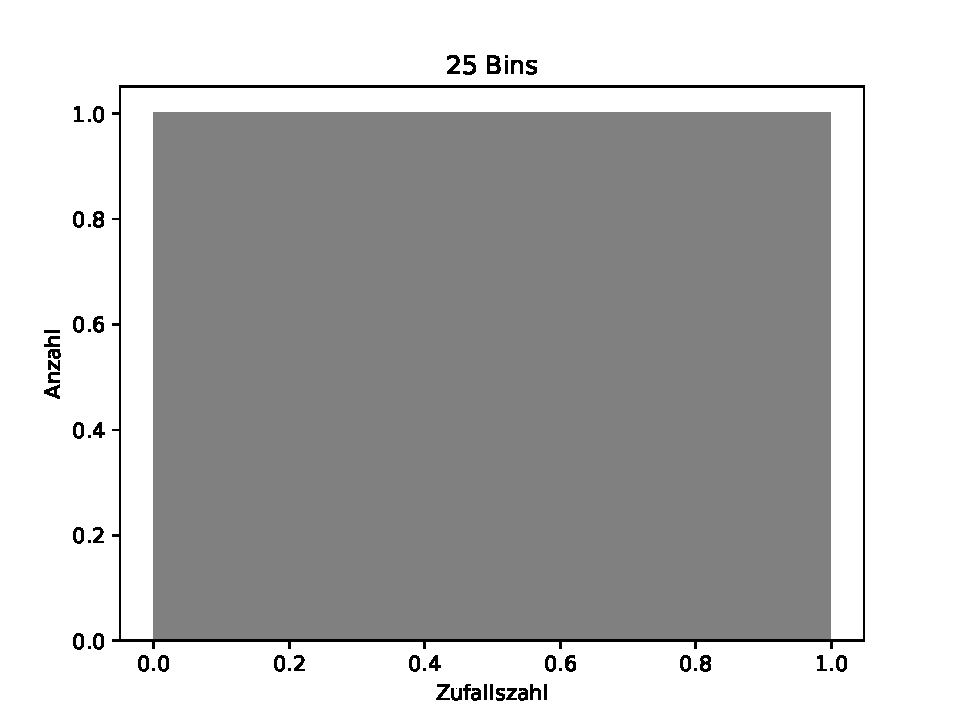
\includegraphics{Aufgabe06/Teilaufgabe_b)_Histogramm.pdf}
  \caption{Histogramm der Zufallswerte}
  \label{fig:6bhist}
\end{figure}
Das in \ref{fig:6bhist} zu sehende Ergebnis ist für Zufallszahlengeneratoren gut, da keine Zahl (viel) öfter gezogen wird, als eine andere.

\subsection{Teilaufgabe c)} \label{sec:6c}
Für die gegeben Startwerte ergeben sich folgende Scatter-Plots:
\begin{figure}[H]
  \centering
  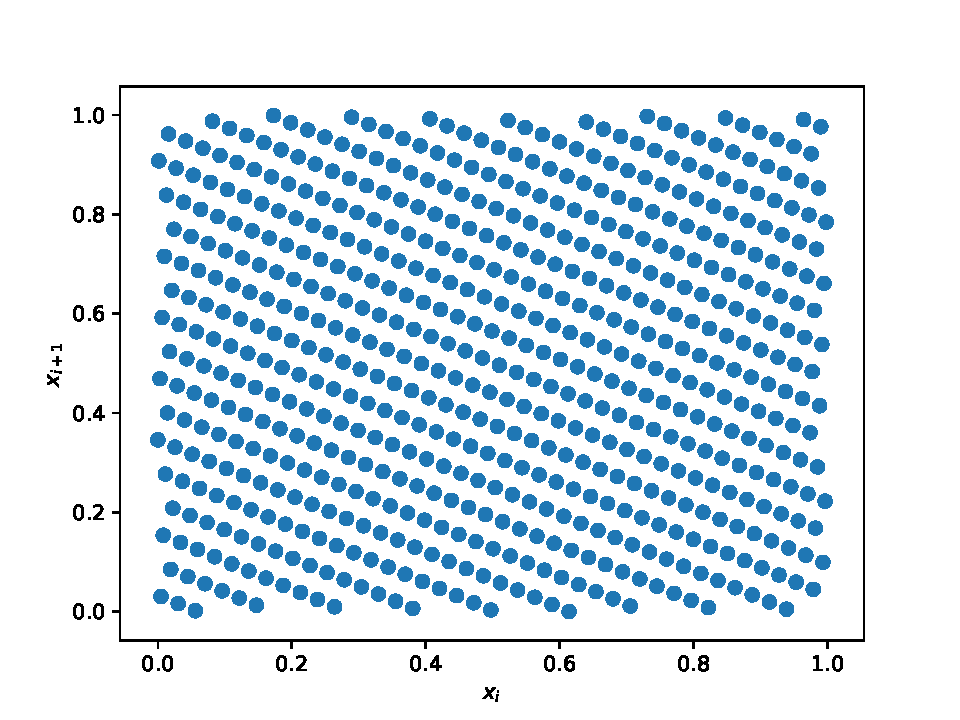
\includegraphics[width=0.7\textwidth]{Aufgabe06/Teilaufgabe_c)_2D-Scatter.pdf}
  \caption{2D-Scatter}
  \label{fig:2dscatterd}
\end{figure}

\begin{figure}[H]
  \centering
  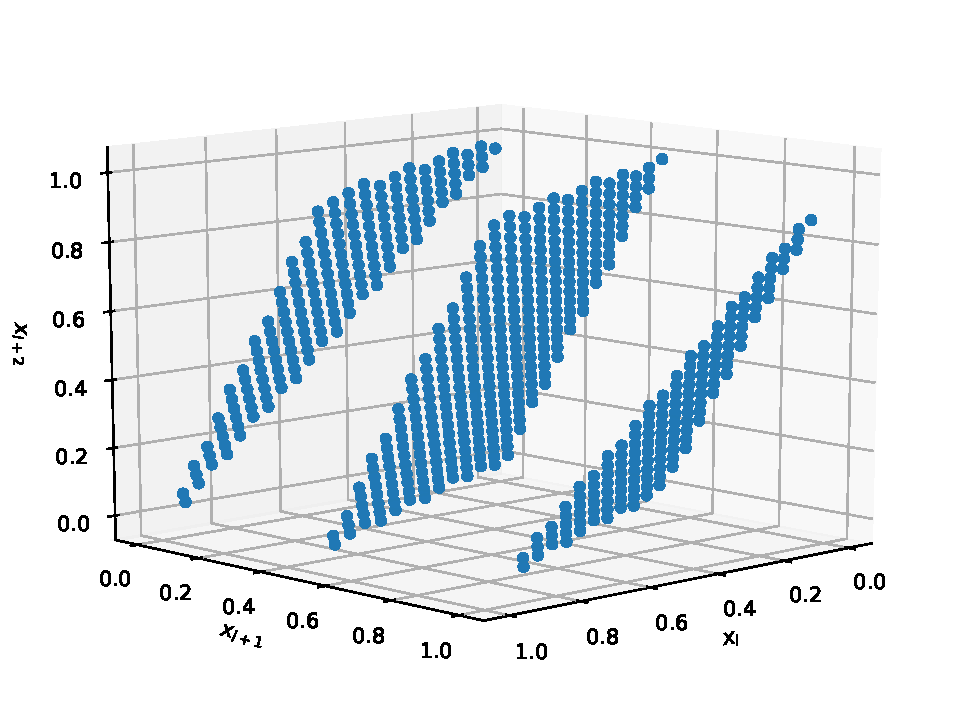
\includegraphics[width=0.7\textwidth]{Aufgabe06/Teilaufgabe_c)_3D-Scatter.pdf}
  \caption{3D-Scatter}
  \label{fig:3dscatterd}
\end{figure}
Da sich in beiden Plots Regelmäßigkeiten erkennen lassen, handelt es sich um keinen guten Zufallszahlengenerator.

\subsection{Teilaufgabe d)}
In dieser Teilaufgabe werden die Ergebnisse aus \ref{sec:6b} und \ref{sec:6c} mit \textit{numpy.random.uniform(0, 1)} verglichen.
Damit die Ergebnisse rekonstruierbar sind, wurde als Seed \textit{np.random.seed(42)} gewählt.
Für die Funktion \textit{numpy.random.uniform(0, 1)} ergibt sich folgendes Histogramm:
\begin{figure}[H]
  \centering
  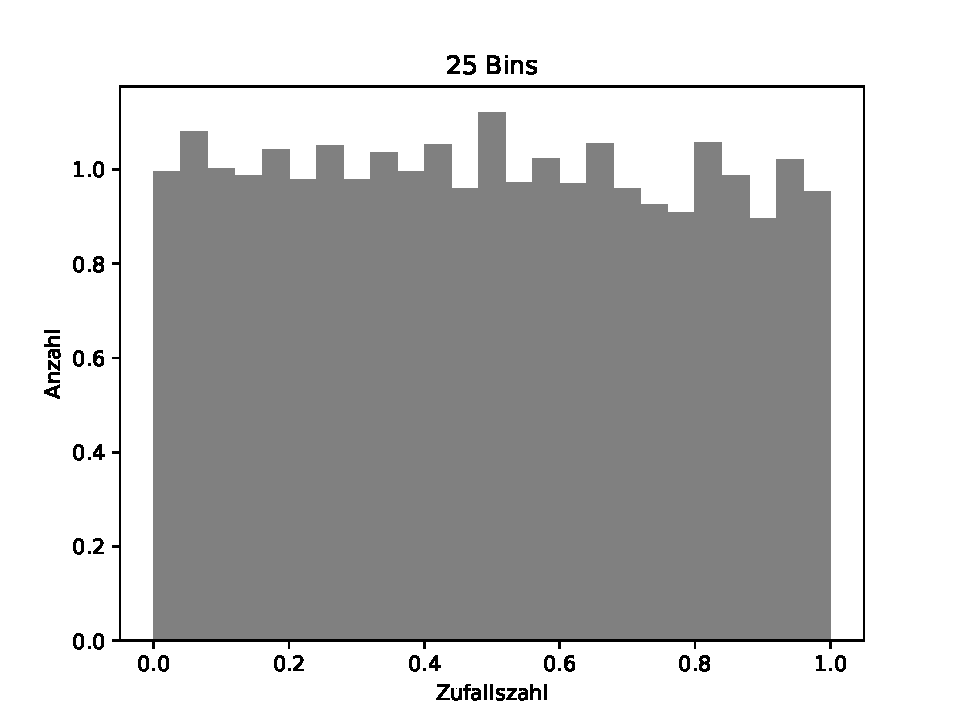
\includegraphics[width=0.7\textwidth]{Aufgabe06/Teilaufgabe_d)_Histogramm.pdf}
  \caption{Histgrogramm für \textit{numpy.random.uniform(0, 1)}}
  \label{6dhist}
\end{figure}
Im Vergleich mit \ref{6bhist} fällt auf, dass die Zufallszahlen weniger gleichverteilt sind, was den Zufallsgenerator in dieser Hinsicht etwas schlechter macht.
Es ergeben sich folgende Scatter-Plots:
\begin{figure}[H]
  \centering
  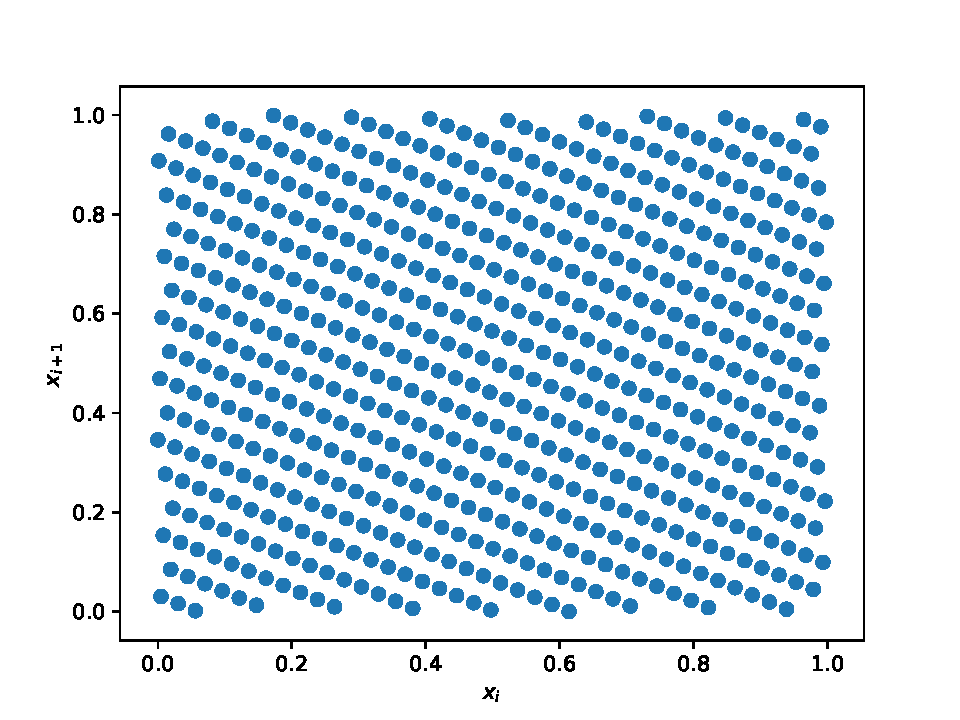
\includegraphics[width=0.7\textwidth]{Aufgabe06/Teilaufgabe_c)_2D-Scatter.pdf}
  \caption{2D-Scatter}
  \label{fig:2dscatterc}
\end{figure}

\begin{figure}[H]
  \centering
  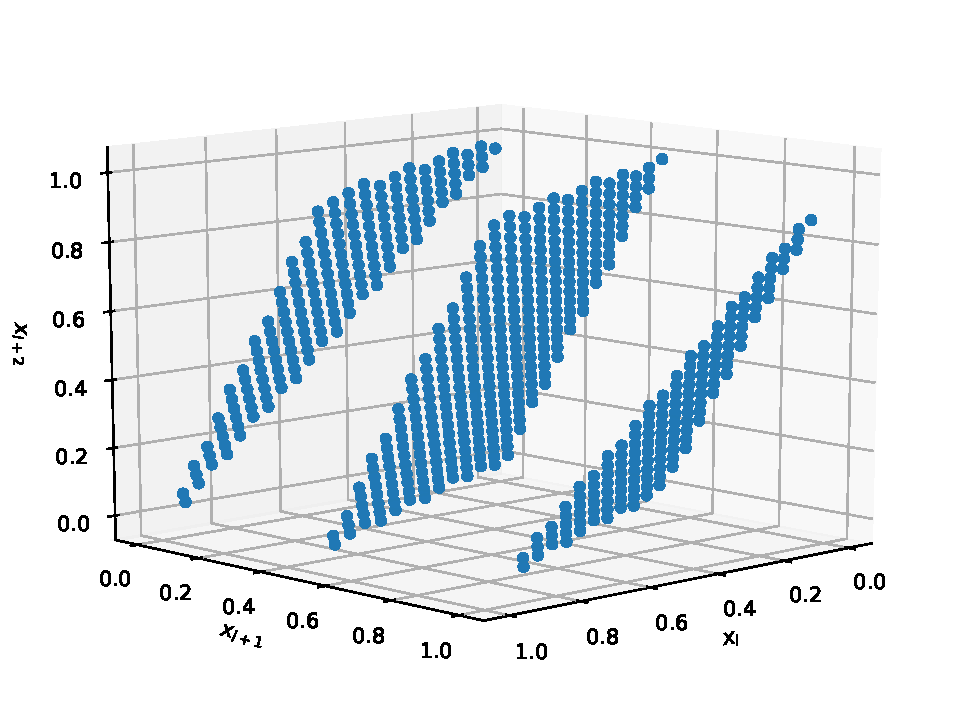
\includegraphics[width=0.7\textwidth]{Aufgabe06/Teilaufgabe_c)_3D-Scatter.pdf}
  \caption{3D-Scatter}
  \label{fig:3dscatterc}
\end{figure}

Im Vergleich zu \ref{fig:2dscatterc} und \ref{fig:3dscatterc} fällt hier jedoch auch, dass die Zufallszahlen hier "zufälliger" verteilt sind und sich kein Gitter erkennen lässt, womit \textit{numpy.random.uniform(0, 1)} in dieser Hinsicht besser ist.

\subsection{Teilaufgabe e)}
Für ganzzahlige $x_0$ liefert der Zufallsgenerator den Wert $\frac{1}{2}$ genau 1 mal (pro Periode).
Für nicht-ganzzahlige $x_0$ tritt dieser Wert nicht auf.
